\section{Ejercicio 2}

Para este ejercicio se pedía ejecutar y graficar usando el algoritmo \textbf{FCFS} para 1, 2 y 4 núcleos, con un cambio de contexto de 2 ciclos, para la tarea (\emph{ej2lote}): 

\begin{center}
	\begin{tabular}{|l|}
		\hline
		TaskCPU 10			\\
		@5:					\\
		TaskConsola 5 1 4	\\
		@6:					\\
		TaskConsola 5 1 2	\\
		@8:					\\
		TaskCPU 10			\\
		\hline
	\end{tabular}
\end{center}

Los gráficos en cuestión son:

\begin{figure}[!h]
	\begin{center}
		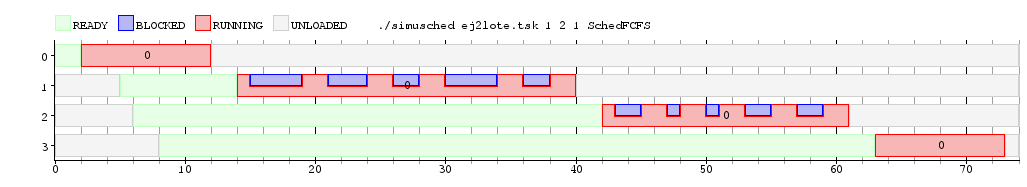
\includegraphics[width=500px]{imagenes/ej2_1.png}
		\caption{Ejecución del lote \emph{ej2lote} con 1 núcleo.}
		\label{fig:grafico_ej2_1}
	\end{center}
\end{figure}

\begin{figure}[!h]
	\begin{center}
		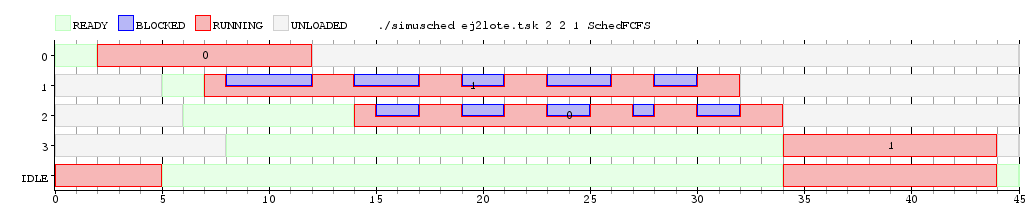
\includegraphics[width=500px]{imagenes/ej2_2.png}
		\caption{Ejecución del lote \emph{ej2lote} con 2 núcleos.}
		\label{fig:grafico_ej2_2}
	\end{center}
\end{figure}

\begin{figure}[!h]
	\begin{center}
		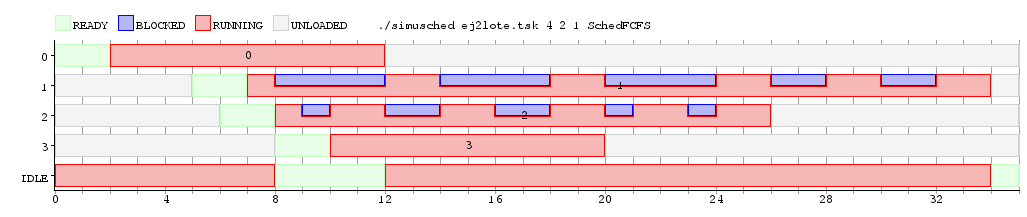
\includegraphics[width=500px]{imagenes/ej2_4.png}
		\caption{Ejecución del lote \emph{ej2lote} con 4 núcleos.}
		\label{fig:grafico_ej2_4}
	\end{center}
\end{figure}

\newpage

\subsection{Latencia} \label{ej2_latencia}

Con los gráficos obtenidos procedemos a calcular la \emph{latencia} de los procesos ejecutados en el scheduler en cuestión.

Ésta consiste en el tiempo en que el proceso tarda en comenzar a ejecutarse una vez que el proceso fue cargado en el scheduler.

Realizamos el calculo de la misma:

\begin{center}
	\begin{tabular}{|c|c|c|c|c|}
		\hline
		\multicolumn{5}{|c|}{\large{\textbf{Latencia}}} \\
		\hline
		\textbf{Cant. Nucleos} & \textbf{TaskCPU @0} & \textbf{TaskConsola @5} & \textbf{TaskConsola @6} & \textbf{TaskCPU @8} \\
		\hline
		1 & 2 & 9 & 36 & 55 \\
		2 & 2 & 2 & 8 & 26 \\
		4 & 2 & 2 & 2 & 2 \\
		\hline
	\end{tabular}
\end{center}


\subsection{Throughput}

Con los mismos gráficos ahora calculamos el \emph{throughput} que consiste en la cantidad de procesos que terminan por unidad de tiempo.

El \emph{throughput} obtenido es:
\begin{figure}[!h]
	\begin{center}
		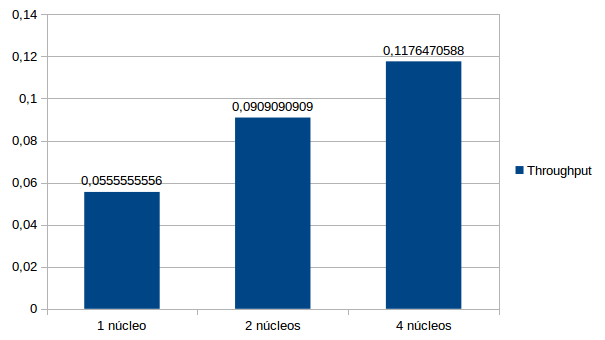
\includegraphics[width=250px]{imagenes/ej2_throughput.png}

		\label{fig:grafico_ej2_throughput}
	\end{center}
\end{figure}

Como se puede observar en el gráfico, el throughput se incrementa a medida de que aumenta la cantidad de núcleos.

